\documentclass{article}\usepackage[]{graphicx}\usepackage[]{color}
%% maxwidth is the original width if it is less than linewidth
%% otherwise use linewidth (to make sure the graphics do not exceed the margin)
\makeatletter
\def\maxwidth{ %
  \ifdim\Gin@nat@width>\linewidth
    \linewidth
  \else
    \Gin@nat@width
  \fi
}
\makeatother

\definecolor{fgcolor}{rgb}{0.345, 0.345, 0.345}
\newcommand{\hlnum}[1]{\textcolor[rgb]{0.686,0.059,0.569}{#1}}%
\newcommand{\hlstr}[1]{\textcolor[rgb]{0.192,0.494,0.8}{#1}}%
\newcommand{\hlcom}[1]{\textcolor[rgb]{0.678,0.584,0.686}{\textit{#1}}}%
\newcommand{\hlopt}[1]{\textcolor[rgb]{0,0,0}{#1}}%
\newcommand{\hlstd}[1]{\textcolor[rgb]{0.345,0.345,0.345}{#1}}%
\newcommand{\hlkwa}[1]{\textcolor[rgb]{0.161,0.373,0.58}{\textbf{#1}}}%
\newcommand{\hlkwb}[1]{\textcolor[rgb]{0.69,0.353,0.396}{#1}}%
\newcommand{\hlkwc}[1]{\textcolor[rgb]{0.333,0.667,0.333}{#1}}%
\newcommand{\hlkwd}[1]{\textcolor[rgb]{0.737,0.353,0.396}{\textbf{#1}}}%

\usepackage{framed}
\makeatletter
\newenvironment{kframe}{%
 \def\at@end@of@kframe{}%
 \ifinner\ifhmode%
  \def\at@end@of@kframe{\end{minipage}}%
  \begin{minipage}{\columnwidth}%
 \fi\fi%
 \def\FrameCommand##1{\hskip\@totalleftmargin \hskip-\fboxsep
 \colorbox{shadecolor}{##1}\hskip-\fboxsep
     % There is no \\@totalrightmargin, so:
     \hskip-\linewidth \hskip-\@totalleftmargin \hskip\columnwidth}%
 \MakeFramed {\advance\hsize-\width
   \@totalleftmargin\z@ \linewidth\hsize
   \@setminipage}}%
 {\par\unskip\endMakeFramed%
 \at@end@of@kframe}
\makeatother

\definecolor{shadecolor}{rgb}{.97, .97, .97}
\definecolor{messagecolor}{rgb}{0, 0, 0}
\definecolor{warningcolor}{rgb}{1, 0, 1}
\definecolor{errorcolor}{rgb}{1, 0, 0}
\newenvironment{knitrout}{}{} % an empty environment to be redefined in TeX

\usepackage{alltt}
\usepackage[english]{babel}
\IfFileExists{upquote.sty}{\usepackage{upquote}}{}
\begin{document}
\title{Marsh Elevation Monitoring\\
The Nature Conservancy, \\
Long Island NY}
\author{Nicole Maher \& Adam Starke}
\maketitle\thispagestyle{empty}





\section{Intro}
The following is a quick compilation of the trends that have been measured at sites being monitored by TNC across Long Island. Note that data is not complete and still needs to be verified fully. The rate of the overall change in elevation is calcuated by finding the average change in each of 9 pins from the start of the monitoring period to the present. More directly, a linear regression is fit to the height of the pins through time. These lines are then averaged across stations for each site. 

Project area:


{\centering 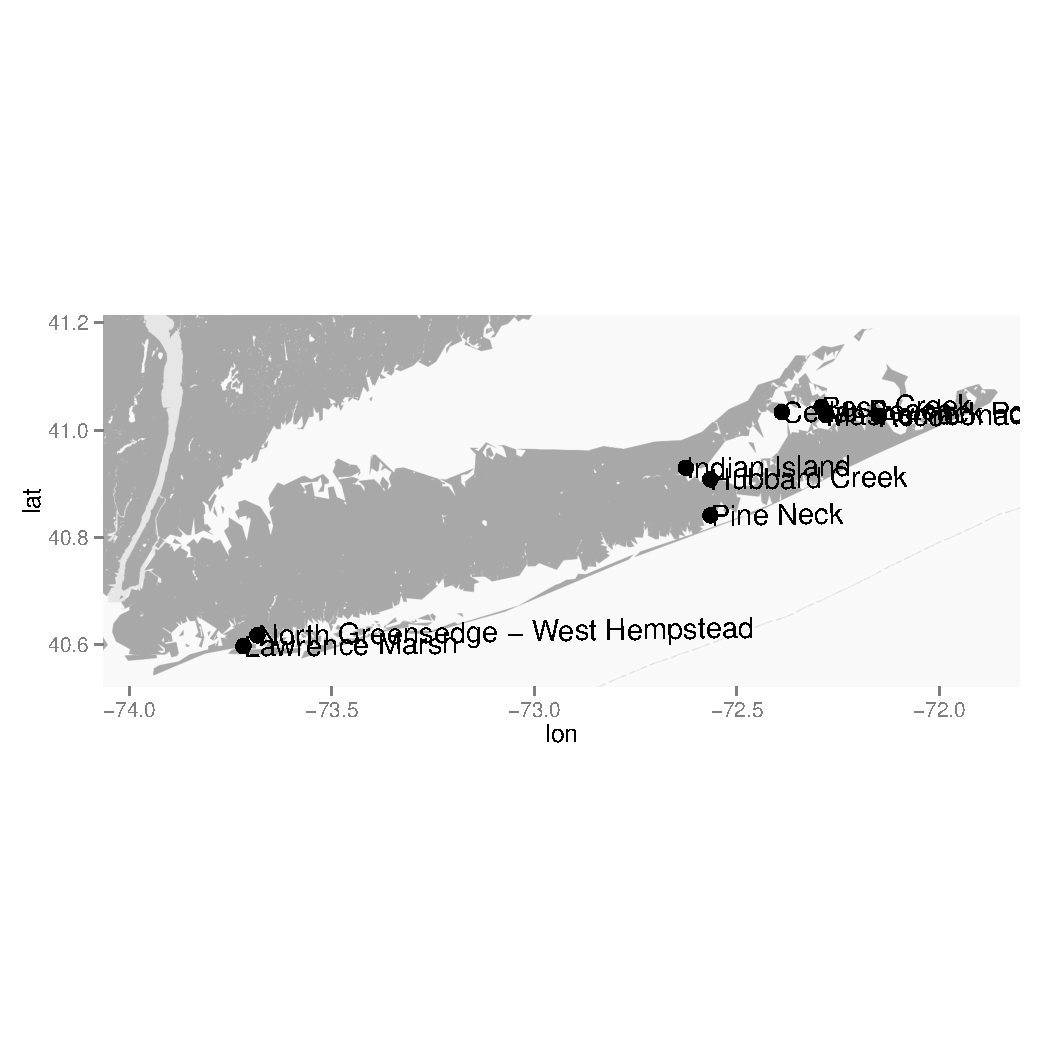
\includegraphics[width=\maxwidth]{figure/Maps} 

}




Tables:
% latex table generated in R 3.0.2 by xtable 1.7-3 package
% Thu Apr 03 13:31:23 2014
\begin{table}[ht]
\centering
\begin{tabular}{rllrrrrrr}
  \hline
 & Site\_Name & Stratafication & Sample N & Mean\_Accretion\_Rate & SE\_ofmeanAccrate & Mean\_elevation\_change & SE\_ofmeanrate & SubSurface\_change \\ 
  \hline
1 & Accobonac Harbor & Low Marsh &  14 & 2.43 & 0.28 & 3.14 & 0.29 & 0.71 \\ 
  2 & Bass Creek & Low Marsh &  15 & 5.54 & 0.26 & 3.45 & 1.61 & -2.08 \\ 
  3 & Cedar Beach & Low Marsh &   9 & 8.73 & 0.39 & 3.79 & 1.70 & -4.95 \\ 
  4 & Hubbard Creek & Low Marsh &  13 & 4.05 & 0.69 & 3.18 & 0.37 & -0.87 \\ 
  5 & Indian Island & High Marsh &   9 & 2.74 & 0.66 & 2.58 & 0.19 & -0.15 \\ 
  6 & Indian Island & Low Marsh &   9 & 4.48 & 0.18 & 3.68 & 0.14 & -0.80 \\ 
  7 & Lawrence Marsh & Low Marsh &   2 &  &  & 4.63 & 1.71 &  \\ 
  8 & Mashomack Point & Low Marsh &   9 & 7.99 & 0.14 & 4.54 & 2.22 & -3.46 \\ 
  9 & North Greensedge - West Hempstead & Low Marsh &   2 &  &  & 3.53 & 2.99 &  \\ 
  10 & Pine Neck & High Marsh &   8 & 4.43 & 0.35 & 4.73 & 0.13 & 0.30 \\ 
  11 & Pine Neck & Low Marsh &   8 & 8.46 & 1.52 & 6.73 & 0.73 & -1.73 \\ 
   \hline
\end{tabular}
\caption{SET-MH monitoring sites across Long Island} 
\end{table}




\section{Visuals}
What follows is a quick visual of the changes that have been measured along the marsh surfaces. The rate of the overall change in elevation is calcuated by finding the average change in each of 9 pins from the start of the monitoring period to the present. More directly, a linear regression is fit to the height of the pins through time. These lines are then averaged across stations for each site. 



{\centering 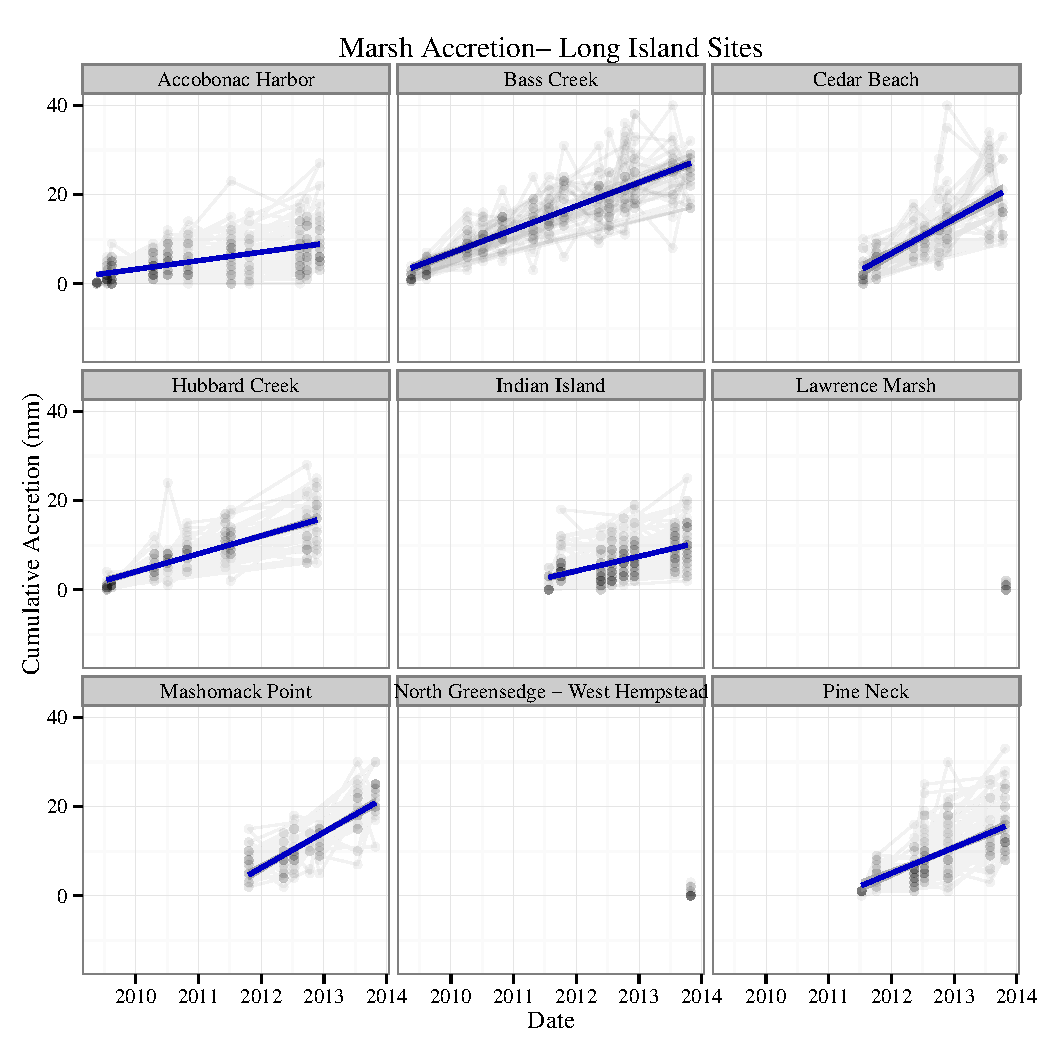
\includegraphics[width=\maxwidth]{figure/SA_Plots} 

}







{\centering 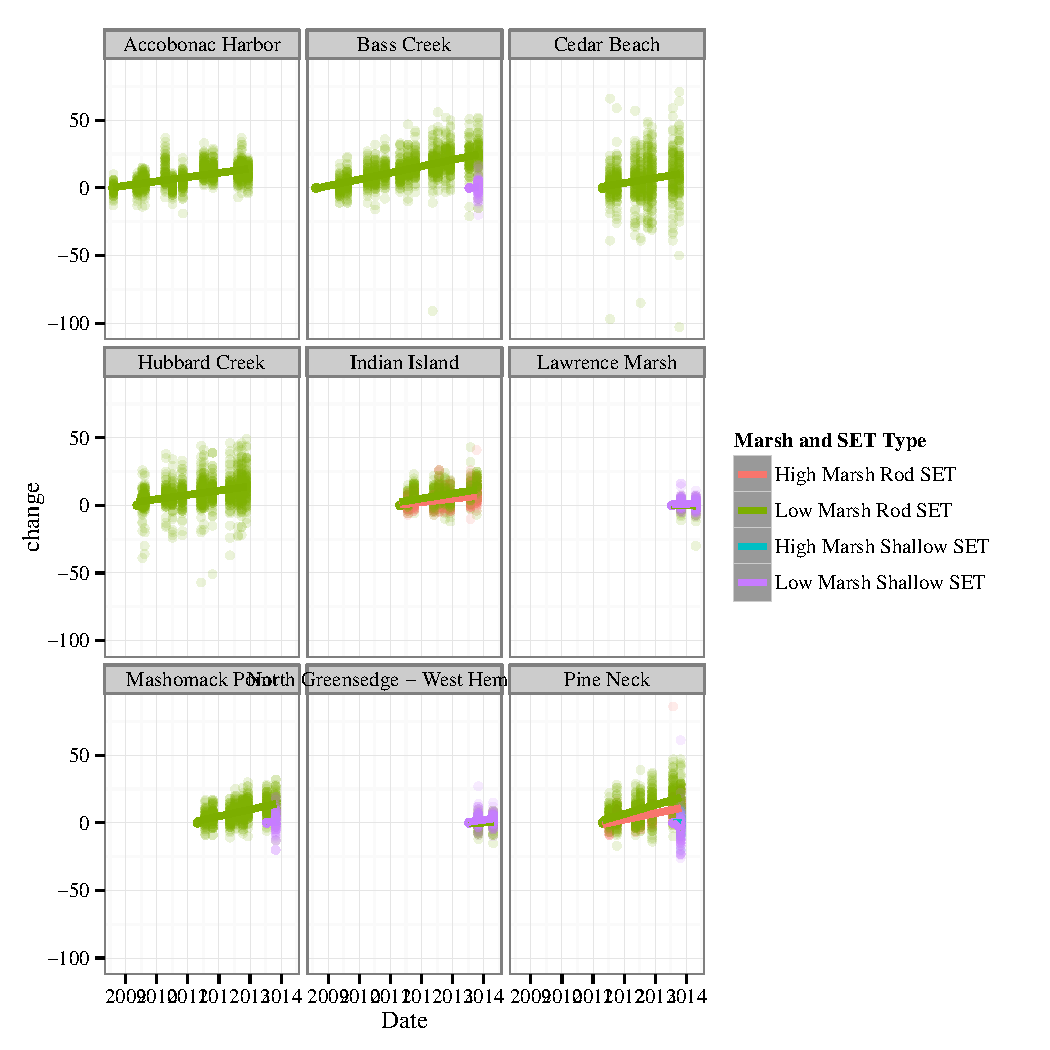
\includegraphics[width=\maxwidth]{figure/Plot_multiLMs} 

}







\end{document}
